\NeedsTeXFormat{LaTeX2e}[1995/12/01]
\documentclass[10pt]{bmc_article}   

% Load packages
\usepackage[ruled,noline]{algorithm2e}
\usepackage{cite} % Make references as [1-4], not [1,2,3,4]
\usepackage{url}  % Formatting web addresses 
\usepackage{ifthen}  % Conditional
\usepackage{multicol}   %Columns
\usepackage[utf8]{inputenc} %unicode support
%\usepackage[applemac]{inputenc} %applemac support if unicode package fails
%\usepackage[latin1]{inputenc} %UNIX support if unicode package fails
\urlstyle{rm}

\def\includegraphic{}
\def\includegraphics{}

\setlength{\topmargin}{0.0cm}
\setlength{\textheight}{21.5cm}
\setlength{\oddsidemargin}{0cm}
\setlength{\textwidth}{16.5cm}
\setlength{\columnsep}{0.6cm}

\newboolean{publ}

%Review style settings
\newenvironment{bmcformat}{\begin{raggedright}\baselineskip20pt\sloppy\setboolean{publ}{false}}{\end{raggedright}\baselineskip20pt\sloppy}

%Publication style settings
%\newenvironment{bmcformat}{\fussy\setboolean{publ}{true}}{\fussy}

% Begin ...
\begin{document}
\begin{bmcformat}

\title{LUMPY: A probabilistic framework for structural variant discovery}
%%%%%%%%%%%%%%%%%%%%%%%%%%%%%%%%%%%%%%%%%%%%%%
%%                                          %%
%% Enter the authors here                   %%
%%                                          %%
%% Ensure \and is entered between all but   %%
%% the last two authors. This will be       %%
%% replaced by a comma in the final article %%
%%                                          %%
%% Ensure there are no trailing spaces at   %%
%% the ends of the lines                    %%     	
%%                                          %%
%%%%%%%%%%%%%%%%%%%%%%%%%%%%%%%%%%%%%%%%%%%%%%
\author{
Ryan M Layer$^1$\email{Ryan M Layer - rl6sf@virginia.edu}\and
Ira M Hall\correspondingauthor$^{2,3}$
\email{Ira M Hall\correspondingauthor - irahall@virginia.edu}
and
Aaron R Quinlan\correspondingauthor$^{2,3}$
\email{Aaron R Quinlan\correspondingauthor - arq5x@virginia.edu}
}

\address{\iid(1)Department of Computer Science, University of Virginia,
Charlottesville, VA\\
\iid(2)Department of Biochemistry and Molecular Genetics,
University of Virginia, Charlottesville, VA\\
\iid(3)Department of Public Health Sciences and
Center for Public Health Genomics, University of Virginia, Charlottesville, VA
}


\maketitle
\begin{abstract}
%Comprehensive discovery of structural variation (SV) in human genomes from DNA
%sequencing requires the integration of multiple alignment ``signals'' including
%read-pair, split-read and read-depth. However, owing to inherent technical
%challenges, most existing SV discovery approaches utilize only one signal and
%consequently suffer from low sensitivity, especially at low sequence coverage
%and for smaller SVs. We present a novel and extremely flexible probabilistic
%SV discovery framework that is capable of integrating any number of SV
%detection signals including those generated from read alignments or prior
%evidence. We demonstrate improved sensitivity over extant methods by combining
%both paired-end and split-read alignments and emphasize the utility of our
%framework for comprehensive studies of structural variation in often
%heterogeneous tumor genomes. We further discuss the utility of this generic
%approach for probabilistic interpretation of diverse genomic data.
%\paragraph*{Background:}
%Comprehensive discovery of structural variation (SV) in human genomes from DNA
%sequencing requires the integration of multiple alignment signals including
%read-pair, split-read and read-depth. However, owing to inherent technical
%challenges, most existing SV discovery approaches utilize only one signal and
%consequently suffer from reduced sensitivity, especially at low sequence
%coverage and for smaller SVs.
%\paragraph*{Results:}
%We present a novel and extremely flexible probabilistic SV discovery framework
%that is capable of integrating any number of SV detection signals including
%those generated from read alignments or prior evidence.
%\paragraph*{Conclusions:}
%We demonstrate improved sensitivity over extant methods by combining paired-end
%and split-read alignments and emphasize the utility of our framework for
%comprehensive studies
%of structural variation in heterogeneous tumor genomes.
\paragraph*{Background:} Comprehensive discovery of structural variation (SV) in
human genomes from DNA sequencing requires the integration of multiple alignment
signals including read-pair, split-read and read-depth.  In a heterogeneous
mixture of diploid genomes, a rare variant may be covered by only a few reads.
Since reads typically produce only one alignment signal, any SV detection
algorithm that considers a single signal, or considers signals individually,
will be unable to identify variants with a diffuse signal.  However, owing to
inherent technical challenges, most existing SV discovery approaches do not
integrate signals and consequently suffer from reduced sensitivity at low
sequence coverage and for rare SVs.
\paragraph*{Results:} We present a novel and extremely flexible probabilistic SV
discovery framework that is capable of integrating any number of SV detection
signals including those generated from read alignments or prior evidence.  Our
framework facilitates this integration by mapping each SV signal to a common
abstract representation, and then performs all SV prediction operations at this
higher level.  This type of abstraction not only allows for efficient and
natural signal integration, it is easily extended to consider new signals.
\paragraph*{Conclusions:} We demonstrate that integrating paired-end and
split-read signals results in a marked improvement in sensitivity over extant
methods in cases where the SV signal is rare (low coverage, low SV allele
frequency, or both).  We also show that there is no increase in false discovery
rate when integrating signals.   SV detection improvements in these instances
are important in clinical settings where it is especially important to identify
variants present in only a small portion of cells in a sample.

\end{abstract}

\ifthenelse{\boolean{publ}}{\begin{multicols}{2}}{}

%%%%%%%%%%%%%%%%%%%%%%
% Introduction
%%%%%%%%%%%%%%%%%%%%%%
%\section{Introduction}
\section*{Background}
Differences in chromosome structure are a prominent source of human genetic
variation. These differences are collectively known as structural variation
(SV), a term that encompasses diverse genomic alterations including deletion,
tandem duplication, insertion, inversion, translocation or complex rearrangement
of relatively large (e.g., $>$100 bp) segments. While SVs are considerably less
common than smaller-scale forms of genetic variation such as single nucleotide
polymorphisms (SNPs), they have much greater functional potential due to their
larger size, and they are more likely to alter gene structure or dosage.
%Indeed, \emph{de novo} SVs contribute to numerous sporadic human disorders,
%polymorphic SVs are increasingly found to be associated with common disease,
%and tumor ``driver'' mutations often arise through gene amplification,
%deletion or fusion.

Our current understanding of the prevalence and impact of SV has
been driven by recent advances in genome sequencing. However, the discovery and
genotyping of SV from DNA sequence data has lagged far behind SNPs because it is
fundamentally more more complicated. SVs vary considerably in size, architecture
and genomic context, and read alignment accuracy is compromised near SVs by the
presence of novel junctions (i.e., breakpoints) between the ``sample'' and
reference genomes. Moreover, SVs generate multiple alignment signals including
altered sequence coverage within duplications or deletions (read-depth),
breakpoint-spanning paired-end reads that align discordantly relative to each
other (paired-end), and breakpoint-containing single reads that align in split
fashion to discontiguous loci in the reference genome (split-reads). These
diverse alignment signals are difficult to integrate and most algorithms use
just one. Other methods use two signals, but to our knowledge these limit
initial detection to one signal and use the other to add confidence, refine
breakpoint intervals, or genotype additional
samples~\cite{rausch2012b,sindi2012,handsaker2011}. The main consequence of
limiting detection to one signal is reduced sensitivity.  The impact of this is
particularly acute in low coverage datasets or in studies of heterogeneous
cancer samples where any given rearrangement may only be present in a small
subset of cells.

% Here, we present a novel probabilistic SV discovery framework that
% naturally integrates multiple SV detection signals, including those generated
% from read alignments or prior evidence, and that can readily adapt to any
% additional source of evidence that may become available with future
% technological advances.



%%%%%%%%%%%%%%%%%%%%%%
% Results
%%%%%%%%%%%%%%%%%%%%%%
\section*{Results}
Here, we present a novel and general probabilistic SV discovery framework that
naturally integrates multiple SV detection signals, including those generated
from read alignments or prior evidence, and that can readily adapt to any
additional source of evidence that may become available with future
technological advances.

\subsection*{Overview of the probabilistic framework}

Our probabilistic framework is based upon a general probabilistic representation
of an SV breakpoint that allows any number of SV alignment signals to be
integrated into a single discovery process (Methods). An integrative approach
allows for more sensitive SV discovery than methods that examine merely one
signal, especially when considering heterogenouse samples and low coverage data,
because each individual read generally produces only one signal type (e.g.,
read-pair or split-read, but not both). Moreover, even with high coverage data,
integration of multiple signals can increase specificity by allowing for more
stringent criteria for reporting a variant call.

We define a breakpoint as a pair of bases that are adjacent in a sample genome
but not in a reference genome. To account for the varying level of noise
inherent to different types of alignment evidence, we represent a breakpoint
with pair of probability distributions spanning the predicted breakpoint regions
(Figure 1, Methods). Each position in the two intervals is assigned a
probability that represents the relative likelihood that the given position
represents one end of the breakpoint.

Our framework provides distinct modules that map signals from each alignment
evidence type to our common probability interval pair.  For example, paired-end
sequence alignments are projected to a pair of intervals upstream or downstream
(depending on orientation) of the mapped ends (Figure 1).  The size of the
intervals and the likelihood at each position is based on the empirical size
distribution of the sample's DNA fragment library.  The distinct advantage of
this approach is that \emph{any} type of evidence can be considered, as long
there exists a direct mapping from the alignment signal to breakpoint
likelihoods.  Here we provide three modules for converting SV alignment signals
to breakpoint likelihood intervals: paired-end, split-read, and generic.  We
emphasize that our framework is extensible to possible new alignment signals
from forthcoming DNA sequencing technologies \cite{clarke2009}. The paired-end
module maps the output of a paired-end sequence alignment algorithm
(e.g., novoalign~\cite{hercus2013} or BWA~\cite{li2009a}), the split-read module
maps the output of a split-read sequence alignment algorithm (e.g.,
YAHA\cite{faust2012} or BWA-SW\cite{li2010}), and the generic module allows
users to include SV signal types that do not have a specific module implemented
(e.g., \emph{a priori} knowledge such as known SV, and/or output from
copy-number variation discovery tools).

Once all of the evidence from the different classes is mapped to breakpoint
intervals, all breakpoints with overlapping intervals are clustered and
the probability intervals are integrated to refine the evidence for
rearrangement and the predicted breakpoint interval (see Methods for details). 
Any clustered breakpoint region that contains sufficient evidence (based on
user-defined arguments) is returned as predicted SV. 
Similar to the breakpoint probability, the clustered probabilities give the
relative likelihood of a breakpoint.  The resolution of the predicted breakpoint
regions is improved by trimming the positions with probabilities
in the lower (e.g., the lowest 5 percent) percentile of the distribution.

We have implemented this framework into an open source C++ software package
(LUMPY, available at {\tt https://github.com/arq5x/lumpy-sv})
that is capable of detecting SV from multiple alignment signals in BAM
alignment~\cite{li2009b} files from one or more samples. 

%\begin{figure}
%\center{
%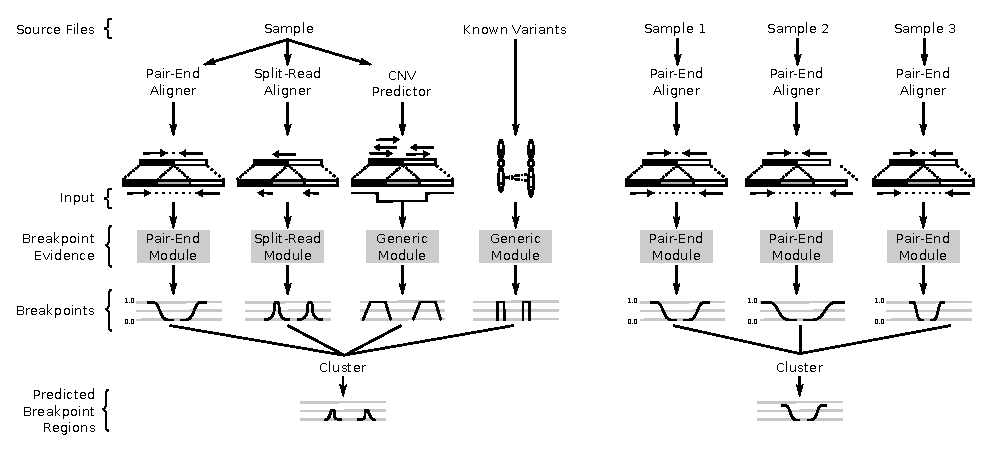
\includegraphics{img/Workflow.eps}
%}
%\caption{The LUMPY probabilistic SV discovery framework with two example
%workflows are presented. One workflow (left) uses three different signals
%(paired-end, split-read, and read-depth) from one sample, as well as prior
%knowledge regarding known variant sites. The second workflow (right) integrates
%a single signal type (in this case, paired-end) from three different samples to
%improve discovery among sensitivity among all three samples.}
%\label{workflow:fig}
%\end{figure}

\subsection*{Comparison of discovery performance on simulated datasets}
Purely homogeneous DNA samples are rare, especially in a clinical setting where
biopsied samples include a mixture of both abnormal and normal tissue.  To
assess the performance of our framework in this realistic scenario, we simulated
heterogeneous samples by pooling reads from an ``abnormal'' genome and a
``normal'' genome at varying ratios.  The source of the simulated abnormal
genome was the human reference genome (build 37) modified (using
SVsim~\cite{faustunpub}) with 5516 non-overlapping deletions identified by the
1000 Genomes Project.  The  source of the simulated normal genome was unmodified
human reference genome (build 37).  Each genome was ``sequened'' using the
paired-end read simulator WGSIM~\cite{liunpub}, and the reades freom the two
genomes were combined to create a single heterogeneous sample.  The ratio of the
reads in a heterogenous sample that are from the abnormal genome (SV allele
frequency) varied between 5\% and 50\%, and the total coverage ranged from 10x
and 80x.  For example, to simulate a sample with a 5\% SV allele frequency at
10x coverage, the affected genome was sequenced at 0.5x coverage and the
unaffected genome at 9.5x coverage.  The two sets of reads were then pooled into
a single 10x coverage heterogeneous sample.

To assess the impact coverage, SV type, and SV size have on the performance of
our framework, we simulated a set of experimental genomes using SVsim that
included 1000 deletions, duplications, insertions, and inversions randomly
placed on chromosome 10 of the human genome (build 37).  For each SV type, 
the variant size ranged from 100bp to 10kb.  We used WGSIM to ``sequence'' each
simulated genome at 2x, 5x, 10x, 20x, and 50x haploid coverage.  

%The length of each read was 150bp and the fragments had a median size of 500bp
%with a standard deviation of 50bp.

We compared LUMPY’s sensitivity and false discovery rate to two other SV
discovery packages GASVPro~\cite{sindi2012} and DELLY~\cite{rausch2012b}.
GASVPro and DELLY were selected because both tools are widely used (DELLY is
part of the 1000 Genomes Project analysis), both consider a secondary SV signal
along with paired-end alignments (coverage and unmapped/split-reads,
respectively), and both have demonstrated improvement the popular SV tools
Breakdancer~\cite{chen2009} and HYDRA~\cite{quinlan2010b}. 


%In order to assess the performance of our framework, we compared LUMPY's
%discovery accuracy using paired-end (PE) alignments, split-read (SR)
%alignments, and both signals to three widely used SV discovery packages: HYDRA
%\cite{quinlan2010b}, GASVPRO \cite{sindi2012} and DELLY \cite{rausch2012b}. We
%created a simulated experimental genome by generating 1000 deletions,
%duplications, insertions, and inversions (4000 events total) throughout
%chromosome 10 of the human genome (build 37) using SVsim (G. Faust,
%unpublished).  For each SV event type, half of the variants were less than 1kb
%and the other half were greater than 1kb (see Methods for details).  We used
%the WGSIM (H. Li, unpublished) paired-end read simulator to ``sequence'' the
%simulated genome to 2, 5, and 20 fold haploid coverage (Methods).

\subsection*{Discovery sensitivity}
The predicted SV breakpoints from each discovery approach were compared to the
simulated breakpoints in order to measure each approach’s sensitivity and false
discovery rate (FDR) for both the heterogeneous experiment (Figure 2) and the
homogeneous experiment (Figure 3).

In the heterogeneous experiment, LUMPY is more sensitive than GASVPro and DELLY
in all cases, and has marked improvement when the coverage of the affected
genome is low (either lower coverage, low SV allele frequency, or both).  For
example, at 10x coverage and 20\% SV allele frequency LUMPY detects 30\% of the
SVs, whereas GASVPro and DELLY detect only 9\% and 5\% of the SVs, respectively.
This is an 11-fold increase in sensitivity over the next best method.  In
general, to achieve the same level of sensitivity as LUMPY, GASVPro and DELLY
require evidence of affected allele to occur in a sample at twice the rate that
LUMPY requires.  At 40x coverage LUMPY detects 30\% of variants when the SV
allele frequency is 5\%, while GASVPro and DELLY do not reach this level of
sensitivity (36\% and 33\%, respectively) until the SV allele frequency is 10\%.

In the homogeneous experiment, LUMPY is consistently more sensitive than other
approaches in all cases, has a marked improvement at lower coverage, and can
detect all SV types (GASVPro does detect duplications and DELLY does not detect
insertions).   For example, LUMPY detects 31\% and 79\% of all deletions at 2
and 5 fold genome coverage, whereas GASVPro and DELLY detect 4.3\%/35\% and
3.4\%/38.4\%, respectively.  At lower coverage (i.e., 2 and 5X), LUMPY’s
sensitivity is greater than all other approaches across all SV types. At most,
LUMPY was 9 times more sensitive than the second most sensitive approach at low
coverage (LUMPY 31\% vs. DELLY 3.4\% for deletions at 2X coverage). At worst, it
was 1.01 times more sensitive for inversions at 5X coverage (LUMPY 90\% vs.
GASVPRO 82\%). At higher (20X and 50x) coverage, LUMPY’s sensitivity advantage
persists; it ranges from 90\% to 98.7\% across all SV types, whereas GASVPRO and
DELLY range from 67\% to 93\% and from 82\% to 95\%, respectively (excluding the
SV types which GASVPRO and DELLY are incapable of detecting).  


%Tratiee predicted SV breakpoints from each discovery approach were compared to the
%simulated breakpoints in order to measure each approach's sensitivity (Figure 2)
%and false discovery rate (FDR; Table 1). Not surprisingly, for each approach,
%breakpoint discovery sensitivity increases with greater genome coverage.
%LUMPY's sensitivity is improved when both paired-end and split-read
%alignments are integrated into the probabilistic framework, as compared to
%discovery with either signal alone. In addition, LUMPY is consistently more
%sensitive than other approaches at lower coverage for all SV types. For example,
%LUMPY detects 24.5\% and 79.3\% of all deletions at 2 and 5 fold genome
%coverage, whereas HYDRA, the next most sensitive approach, detects 2.9\% and
%30.9\%, respectively.

%\begin{figure}
%\includegraphics[width=6.5in]{R/ss_sl_s-un_hy_gv_dl-r10x.eps}
%\caption{SV discovery sensitivity for LUMPY, HYDRA, GASVPRO, and DELLY for
%different SV types across multiple genome coverage levels. \emph{lumpy-pe}
%reflects LUMPY sensitivity using \emph{only} paired-end alignments;
%\emph{lumpy-sr} reflects LUMPY sensitivity using \emph{only} split-read
%alignments; \emph{lumpy} describes sensitivity when integrating \emph{both}
%paired-end and split-read alignments; \emph{delly-pe} reflects DELLY sensitivity
%using paired-end alignments only; \emph{delly-sr} reflects DELLY sensitivity
%using paired-end alignments for discovery followed by split-read refinement of
%paired-end SV predictions.}
%\label{sensitivity:fig}
%\end{figure}

%At lower coverage (i.e., 2 and 5X), LUMPY's sensitivity is greater
%than all other approaches across all SV types. At most, LUMPY was
%8.4 times more sensitive than the second most sensitive approach at low
%coverage (LUMPY 24.5\% vs. HYDRA 2.9\% for deletions at 2X coverage). At worst,
%it was 1.3 times more sensitive for inversions at 5X coverage (LUMPY 94.7\% vs.
%GASVPRO 70.9\%). At higher (20X) coverage,
%LUMPY's sensitivity advantage persists; it ranges from 95.2\% to 96.9\%
%across all SV types, whereas HYDRA and GASVPRO range from 76.9\% to 92.8\% and
%59.9\% to 91.9\%, respectively (excluding duplications which GASVPRO is
%incapable of detecting).
%
%Unlike the other tools compared, LUMPY has nearly equal sensitivity for
%both smaller (i.e. \textless 1kb) and larger (\textgreater 1kb) events.
%Whereas at 20X coverage,
%LUMPY detects 95.6\% and 94.6\% of deletions less and greater than 1kb,
%respectively, GASVPRO and HYDRA each have much lower sensitivity for small
%variants than for large (62.3\% vs 97.1\% for HYDRA and 50.7\% and 94.6\% for
%GASVPRO). This increased sensitivity is especially important given that smaller
%SVs are much more common than larger events \cite{mills2011}.
%

\subsection*{False discovery rate}
Improved sensitivity is crucial for comprehensive studies of genome variation,
yet high sensitivity at the cost of an inflated false discovery rate (FDR) is
undesirable given the time and cost associated with pursuing the putative
biological impact of spurious variation.

We compared the FDR for each SV discovery tool using the same simulated
SVs as described above (Table 1).The false discovery rate for all tools ranged
from 0.0\% to 24.2\%. Overall, DELLY-SR had the lowest FDR across all SV types
and genome coverage levels, yet the conservative calling comes at the cost of
lower sensitivity compared to the other tools. While LUMPY's FDR was
slightly higher than GASVPRO for deletions, its FDR was consistently
low (0.0\% - 5.0\%) across all SV types and coverage levels. In contrast,
GASVPRO had much higher FDRs for insertions and inversions and
its FDR increased at lower coverage levels.  HYDRA had consistent FDRs across
SV types and coverage levels (0.0\% to 8.9\%), yet these rates were always
higher than the analogous LUMPY FDRs. These results indicate that LUMPY's
probabilistic framework afford substantial improvements in discovery
sensitivity while maintaining low false discovery rates.

%\begin{table}[h!b!p!]
%\small
%\caption{False discovery rates for each SV discovery approach.}
%\begin{tabular}{l|lll|lll|lll|lll}
%		Coverage
%		&20x&5x&2x &20x&5x&2x &20x&5x&2x &20x&5x&2x \\
%\cline{1-13}
%			Variety
%			&\multicolumn{3}{c}{Deletions}
%			&\multicolumn{3}{|c}{Duplications}
%			&\multicolumn{3}{|c}{Insertions}
%			&\multicolumn{3}{|c}{Inversions} \\
%\cline{1-13}
%lumpy-pe		&0.014&0.008&0&0.004&0	  &0    &0.042&0.016&0	  &0.004&0	  &0 \\
%lumpy-sr      &0.006&0	&0&0.005&0.003&0	&0.013&0.006&0	  &0.004&0.001&0 \\
%lumpy    &0.018&0.005&0&0.007&0.001&0	&0.05 &0.009&0	  &0.009&0.002&0 \\
%hydra   &0.038&0.006&0&0.03 &0.011&0	&0.089&0.034&0.03 &0.054&0.006&0 \\
%gasvpro	&0	  &0	&0&N/A  &N/A  &N/A  &0.242&0.065&0.041&0.005&0.082&0.079 \\
%delly-pe	&0.002&0	&0&0	&0	  &0.028&N/A  &N/A	&N/A  &0	&0	  &0 \\
%delly-sr	&0	  &0	&0&0	&0	  &0	&N/A  &N/A	&N/A  &0.004&0	  &0 \\
%
%\end{tabular}
%\label{table:fdr}
%\end{table}


\subsection*{Benefits of integrating all signals for SV discovery}

LUMPY's increased sensitivity is driven by the fact that both paired-end and
split-read signals are combined during SV discovery. More generally, our
framework is capable of pooling any number of signals in order to further
increase sensitivity. To our knowledge, while other tools exploit multiple SV
signals, they first exploit one signal to drive discovery and then refine
candidates with a second signal. An intrinsic limitation of such stepwise
approaches is other available signals cannot increase the number of true
positive SV calls beyond those candidates identified by the signal used for
initial discovery. DELLY, for example, uses split-read alignment strategies to
refine candidate variants identified via graph ``cliques'' of discordant
paired-end alignments~\cite{rausch2012b}. As illustrated in Figure 2, DELLY's
sensitivity is reduced when examining both SV signals in stepwise fashion,
whereas LUMPY's sensitivity increases when both signals are integrated. The
impact on sensitivity is especially dramatic at lower sequence depth: at 2X
coverage, DELLY's deletion sensitivity is reduced by 60\%, while LUMPY's
sensitivity increased six-fold when integrating both signals.

It is well-known that variant calling is improved by integrating data from
multiple samples~\cite{handsaker2011, mckenna2010, hormozdiari2011,
quinlan2011}, especially when searching for mutations that are rare or private
to a single sample. The LUMPY framework naturally handles multiple samples by
tracking the sample origin of each probability distribution during clustering.
Given that LUMPY can analyze a single human dataset (HG00262 from the 1000
Genomes Project) comprising 104 million read pairs in less than an hour with one
thread, we anticipate that simultaneous analysis of tens to hundreds of genomes
will be possible with LUMPY using commodity hardware.

Furthermore, by integrating multiple signals, the resolution of our
predicted breakpoint intervals is increased relative to the resolution yielded
by examining either signal on its own. For example, at 20X coverage, use of both
signals refines deletion breakpoint predictions to within a median of 5 bp of
the true location. When paired-end alignments alone drive discovery, our
breakpoint resolution is reduced by more than 50 fold (median of 265 bp) and as
expected, this increase in resolution is observed across all other SV types
(data not shown).

\section*{Discussion}
We have developed a general probabilistic framework for accurate SV discovery,
and have demonstrated that our framework is more sensitive than existing
discovery tools across all SV types and coverage levels. Importantly, the
increased sensitivity does not come at the cost of excessive spurious SV
predictions.

Our framework represents an important technological advance, especially in the
context of cancer genomics where sensitivity is crucial to understanding tumor
evolution. While highly sensitive methods have been developed for point
mutations, similar sensitivity has been challenging for structural variation
owing to the technical challenges inherent to characterizing genomic
rearrangements from DNA sequence alignments. Our approach greatly simplifies the
problem by providing a common framework for representing and integrating
breakpoint likelihoods from any number of SV alignment signals. Any signal can
be integrated into our framework so long as a breakpoint likelihood can be
assigned to each base pair in a candidate breakpoint region. The result is a
dramatic increase in SV discovery sensitivity and a corresponding increase in
the resolution of the predicted breakpoint interval.

%We emphasize that the framework's flexibility permits facile improvements to
%sensitivity through the integration of alignment data from multiple samples
%(e.g., tumors and matched normal tissue), as well sites of known rearrangement.
%For example, while our FDR was slightly higher for deletions than other tools,
%integrating copy-number predictions into our calling framework similar to
%GASVPRO (Figure 1; generic module) would bring our deletion FDR to nearly zero.

It has not escaped our notice that this general approach can be used to perform
probabilistic set theory operations on diverse genomic interval datasets. One
immediate application of this framework is interpretation of splicing patterns
from RNA-seq data, where sensitivity for low abundance transcripts is paramount,
and where there is generally prior evidence for breakpoint positions (i.e.,
exons). ChIP-seq is another attractive application, as different ChIP-seq
datasets are typically analyzed through binary comparisons of peak intervals:
that is, do the peaks overlap or not? However, were peaks converted to
probability distributions, multiple datasets could be integrated in a
probabilistic fashion analogous to how LUMPY interprets SV signals, thus
preserving both the spatial and quantitative information underlying the
experiment. As a more powerful alternative to traditional peak finding, we
envision multi-sample data integration using whole-genome probability
distributions, perhaps through extension of existing interval-based software
such as our own BEDTools~\cite{quinlan2010a}. Such toolsets will empower
sophisticated probabilistic analyses of inherently complex and nuanced datasets
such as ENCODE~\cite{encode2012}. In general, our framework applies to any data
type that can be represented as a probability distribution across genome space.


\section*{Methods}

We propose a breakpoint prediction framework that can accommodate multiple
classes of evidence from multiple sources in the same analysis.  To accomplish
this, we define a high-level breakpoint type that represents the consensus
breakpoint location from different pieces of evidence.  Our framework makes use
of an abstract breakpoint evidence type to define a set of functions that serve
as an interface between specific evidence subtypes (e.g., paired-end sequence
alignments and split-read mappings) and the breakpoint type.  Any class of
evidence for which these functions can be defined may be included in our
framework.  To demonstrate the applicability of this abstraction, we defined
three breakpoint evidence subtypes: paired-end sequencing, split-read mapping,
and a general breakpoint interface.

Since our framework combines evidence from multiple classes, it extends
naturally to include evidence from multiple sources.  The sources that can be
considered in a single analysis may be any combination of evidence from
different samples, different evidence subclasses from the same samples, or
data sets from known genomic features.  We refer to a given data set as a
breakpoint evidence instance, and assume that each instance contains only one
evidence subtype and is from a single sample.  To help organize the results of
analysis with multiple samples or multiple instances for a single sample,
each instance is assigned an id that can be shared across instances.


\subsection*{Breakpoint}

A breakpoint is a pair of genomic sequences that are adjacent in a sample genome
but not in a reference genome. Breakpoints can be detected, and their locations
predicted by various evidence classes (e.g., paired-end sequence alignments and
split-read mappings).  To support the inclusion of different evidence classes
into a single analysis, we define a high-level breakpoint type as a collection
of the evidence that corroborates the location and variety of a particular
breakpoint.  Since many evidence classes provide a range of possible breakpoint
locations, we represent the breakpoint's location with a pair of breakpoint
intervals where each interval has a a start position, an end position, and a
probability array that represents the likelihood that a given position in the
interval is one end of the breakpoint.  More formally, a breakpoint is a tuple
$b=\langle E,l,r,v \rangle$ where: $E$ is the set of evidence that corroborates
the location and variety of a particular breakpoint; $l$ and $r$ are left and
right breakpoint intervals each with values $s$ and $e$ that are the start and
end genomic coordinates and $p$ is a probability array where $|p|=e-s$ and
$p[i]$ is the relative probability that position $s+i$ is one end of the
breakpoint; and $v$ is the breakpoint variety (e.g., $\textsc{Deletion}$,
$\textsc{Duplication}$, etc.)

If there exists two breakpoints $b$ and $c$ in the set of all breakpoints $B$
where $b$ and $c$  intersect ($b.r$ intersects $c.r$, $b.l$ intersects $c.r$,
and $b.v = c.v$), then $b$ and $c$ are {\em merged} into interval $m$, $b$ and
$c$ are removed from $B$, and $m$ is placed into $B$.  The evidence set $m.E$ is
the union of the evidence sets $b.E$ and $c.E$.  

A straight-forward method to define breakpoint intervals $m.l$ and $m.r$ would
would be to let $m.l.s = \max(b.l.s, c.l.s)$, $m.l.e = \min(b.l.e, c.l.e)$,
similar for $m.r$.  However, if a spurious alignment is merged into a set
genuine breakpoints, the resulting breakpoint interval can be ``pulled'' away
from the actual breakpoint.  The impact of an outlier can be minimized or
eliminated once the full set of agreeing alignments is collected for a given
breakpoint, but collecting the full set is complicated by the fact that
alignments are considered in-order and outliers typically occur first.  To
account for this, we define a liberal merge process where $m.l.s$ is the mean
start position for the left intervals in $m.E$, and  $m.l.e$ is the mean
end position for the left intervals in $m.E$, similar for $m.r$.

Once all the evidence has been considered, an SV call $s$ is make for each
breakpoint $b\in B$.  The boundaries of the breakpoint intervals $s.l$ and $s.r$
are the trimmed mixture distributions of the left and right intervals in $b.E$.
Let $s.l.s=min( \{e.l.s | e\in b.E\})$, $s.l.e=min( \{e.l.e | e\in b.E\})$, and
$s.l.p[i] = \sum_{e \in b.E} e.l.p[i-o]$ where $o$ is the offset value
$e.l.s-s.l.s$.  Similar for $s.r$.  The value at $s.l.p[i]$ (or $s.r.p[i]$)
represents the level of agreement among the evidence in $b.E$ that position $i$
is one end of the breakpoint.  The intervals $s.l$ and $s.r$ are then trimmed to
include only those positions that are in the top percentile (e.g., top 99.9
percent of values).  An outlier in $b.E$ will extend the interval $s.l$, but the
extended region will have little support from other elements in $b.E$ and values
of $s.p$ in that region will relatively small and are likely to be removed in
the trimming process. 

\subsection*{Breakpoint Evidence}

To combine the distinct SV alignment signals like paired-end and split-read
alignments to the general breakpoint type defined above, we define an
abstract breakpoint evidence type.  This abstract type defines an interface that
allows for the inclusion of any data that can provide the following functions:
$\textsc{is\_bp}$ determines if a particular instance of the data contains
evidence of a break point, $\textsc{get\_v}$ determines the breakpoint variety
(e.g., deletion, duplication, inversion, etc.), and $\textsc{get\_bpi}$
maps the data to a pair of breakpoint intervals.

To demonstrate the applicability of this abstraction, we defined three
breakpoint evidence instances: paired-end sequencing alignments, split-read
mapping, and a general breakpoint interface.  Paired-end sequencing and split
read mapping are among the most frequently used data types for breakpoint
detection, and the general interface provides a mechanism to include any other
breakpoint information such as known breakpoints or output from other analysis
pipelines.  As technologies evolve and our understanding of structural
variations improves, other instances can be easily added.

\subsubsection*{Paired-End Sequencing Alignments}

Paired-end sequencing involves fragmenting genomic DNA into roughly uniformly
sized segments, and sequencing both ends of each segment to produce the sequence
pair $\langle x,y \rangle$.  The ends of the pair are
aligned to a reference genome $R(x)=<o,s,e>$, where $o=+|-$ indicates the
alignment orientation, and $s$ and $e$ delineate the start and end positions of
the matching sequence in the reference genome.  To simply the explanation, we
let the genome be one contiguous interval of concatenated chromosomes so that
all sequences can be referred to by offset only.  Translocations can still be
identified in this model since the positions on different chromosomes will be
far apart.  We also assume that both $x$ and $y$ align uniquely to the
reference and that $R(x).s<R(x).e<R(y).s<R(y).e$.  While it is often not
possible find the exact position of a sequence in the sample genome, it is
useful to refer to $S(x)=<o,s,e>$ as the alignment of $x$ with respect to the
originating sample's genome.

% is_bp
Assuming the reads were made on an Illumina platform, pairs are expected to
align to the reference genome with a $R(x).o=+, R(y).o=-$ orientation, and at
distance $R(y).e - R(x).s$ roughly equivalent to the fragmentation length from
the sample preparation step.  Any pair that aligns with an unexpected
configuration can be evidence of a breakpoint.  These unexpected configurations
include matching orientation $R(x).o = R(y).o$, alignments with switched
orientation $R(x).o=-, R(y).o=+$, and an apparent fragment length ($R(y).e -
R(x).s$) that is either shorter or longer than expected.  We estimated the
expected fragment length to be the sample mean $\overline{l}$ fragment length,
and the fragment length standard deviation to be the sample standard deviation
$\overline{s}$ from the set of properly mapped pairs (as defined by the SAM
spec) in the sample data set.  Considering the variability in the sequencing
process, we extend the expected fragment length to include sizes
$\overline{l}\pm v_l \overline{s}$, where $v_l$ is a tuning parameter that
reflects spread in the data.

The breakpoint variety for $\langle x,y \rangle$ can be inferred from the
orientation that $x$ and $y$ align to in the reference.  If the orientations
match, then the breakpoint was caused by an inversion event, and if the
$R(x).o=-$ and $R(y).o=+$ then there was a duplication event.  When $R(x).o=+$
and $R(y).o=-$, the breakpoint variety is ambiguous between an insertion and a
deletion.  This ambiguity is also true for other types of evidence types (e.g.,
split-read mappings).  While it may be possible to determine which event caused
the breakpoint in a post-processing step, breakpoint correlation is a complex
process and is beyond the scope of this framework.  Since we cannot distinguish
between the two varieties, any pair with a $+/-$ orientation configuration is
marked as a deletion.

To map $\langle x,y \rangle$ to breakpoint intervals $l$ and $r$, the ranges of
possible breakpoint locations must be determined and probabilities assigned to
each position in those ranges.  By convention, $x$ maps to $l$ and $y$ to
$r$, and for the sake of brevity we will focus on $x$ and $l$ since the same
process applies to $y$ and $r$.  Assuming that a single breakpoint exists
between $x$ and $y$, then the sign of $x$ determines if $l$ will be upstream
or downstream of $x$.  If the $R(x).s=+$, then the breakpoint interval begins
after $R(x).e$ (downstream), otherwise the interval ends before $R(x).s$
(upstream). 
%To account for variance in the alignment of $x$, we extend the breakpoint by
%to $R(x).e - v_a$ if $R(x).s=+$ and $R(x).s + v_a$ if $R(x).s=-$,
%where $v_a$ is a turning parameter.

The length of each breakpoint interval is proportional to the expected fragment
length $\overline{l}$ and standard deviation $\overline{s}$.  Since we assume
that only one breakpoint exists is between $x$ and $y$, and that it is unlikely
that the distance between the ends of a pair in the sample genome ($S(y).e -
S(x).s$) is greater than $\overline{l}$, then it is also unlikely that one end
of the breakpoint is at a position greater than $R(x).s + \overline{l}$,
assuming that $R(x).o=+$. If $R(x).o=-$, then it is unlikely that a breakpoint
is at a position less than $R(x).e - \overline{l}$.  To account for variability
in the fragmentation process, we extend the breakpoint to
$R(x).e + (\overline{l} + v_f\overline{s})$ when $R(x).o=+$, and
$R(x).s - (\overline{l} + v_f\overline{s})$ when $R(x).o=-$,
where $v_f$ is a tuning parameter that, like $v_l$, reflects the spread in the
data.

The probability that a particular position $i$ in the breakpoint interval $l$ is
part of the actual breakpoint can be estimated by the probability that $x$ and
$y$ span that position in the sample. For $x$ and $y$ to span $i$, the fragment
that produced $\langle x,y \rangle$ must be longer than then distance from the
start of $x$ to $i$, otherwise $y$ would occur before $i$ and $x$ and$y$ would
not span $i$ (contradiction).  The resulting probability is
$P(S(y).e - S(x).s > i - R(x).s)$ if $R(x).o=+$, and
$P(S(y).e - S(x).s > R(x).e - i)$ if $R(x).o=-$.
While we cannot directly measure the sample fragment length ($S(y).e - S(x).s$),
we can estimate its distribution by constructing a frequency-based cumulative
distribution $D$ of fragment lengths from the same sample that was used to find
$\overline{l}$ and $\overline{s}$, where $D(j)$ gives the proportion of the
sample with fragment length greater than $j$ (Appendix~\ref{pe:sec}
Algorithm~\ref{get_one_bpi} and Algorithm~\ref{get_bpi}).

\subsubsection*{Split-Read Alignments}

A split-read alignment is a single DNA fragment $X$ that does not uniquely align
to the reference genome, but contains a contiguous ordered set of substrings
$(x_1, x_2, \dots, x_n)$ where $X=x_1x_2\dots x_n$, each substring aligns
uniquely to the reference $R(x_i)=\langle o,s,e \rangle$, and adjacent
substrings align to non-adjacent location in the reference genome
$R(x_{i}).e \neq R(x_{i+1}).s + 1$ for $1\leq i \leq n-1$. A single split-read
alignment maps to a set of adjacent split-read sequence pairs
$(\langle x_1 , x_2 \rangle, \langle x_2, x_3 \rangle, \dots ,
\langle x_{n-1},x_n \rangle)$, and each pair $\langle x_i,x_{i+1} \rangle$ is
considered individually.

% is_bp
By definition, a split-read mapping is evidence of a breakpoint and therefore
the function $\textsc{is\_bp}$ trivially returns $\textsc{true}$.

% get_v
Both orientation and mapping location must be considered to infer the breakpoint
variety for $\langle x_i,x_{i+1} \rangle$.  When the orientations match
$R(x_{i}).o=R(x_{i+1}).o$, the event was either a deletion or
a duplication.  Assuming the $R(x_{i}).o=R(x_{i+1}).o=+$,
$R(x_{i}).s<R(x_{i+1}).s$ indicates a gap caused by a deletion and
$R(x_{i}).s>R(x_{i+1}).s$ indicated a repeated sequenced caused by a
duplication.   These observations are flipped when orientations
$R(x_{i}).o=R(x_{i+1}).o=-$.  Similar to paired-end alignments, we do not mark
breakpoints as insertions since we cannot distinguish between deletions
and insertions.  When the orientations do not match $R(x_{i}).o \ne
R(x_{i+1}).o$, the event was an inversion and the mapping locations do not need
to be considered.

% get_bpi
The possibility of errors in the sequencing and alignment processes create some
ambiguity in the exact location of the breakpoint associated with a split-read
sequence pair.  To account for this, each pair $\langle x_i, x_{i+1} \rangle$
maps to two breakpoint intervals $l$ and $r$ centered at the split. The
probability vectors $l.p$ and $r.p$ are highest at the midpoint and
exponentially decreasing toward their edges.  The size of this interval is a
configurable parameter $v_s$ and is based on the quality of the sample under
consideration and the specificity of the alignment algorithm used to map the
sequences to the reference.

Depending the breakpoint variety, the intervals $l$ and $r$ are centered on
either the start or the end of $R(x_i)$ and $R(x_{i+1})$.  When the breakpoint
is a deletion $l$ is centered at $R(x_i).e$ and $r$ at $R(x_{i+1}).s$, and when
the breakpoint is a duplication $l$ is centered at $R(x_i).s$ and $r$ at
$R(x_{i+1}).e$.  If the breakpoint is an inversion, $l$ and $r$ are both
centered either at the start positions or end positions of $R(x_i)$ and
$R(x_{i+1})$, respectively.  Assuming that $R(x_i).s<R(x_{i+1}).s$, if
$R(x_i).o=+$ then $l$ and $r$ are centered at $R(x_i).e$ and  $R(x_{i+1}).e$,
otherwise they are centered at $R(x_i).s$ and  $R(x_{i+1}).s$.  If
$R(x_i).s>R(x_{i+1}).s$, then the conditions are swapped
(Appendix~\ref{sr:sec} Algorithm~\ref{get_bpi_sr}).

\subsubsection*{Generic Evidence}

The generic evidence subclass provides a mechanism to directly encode breakpoint
intervals using the BEDPE format~\cite{quinlan2010a}.  BEDPE is an extension of
the popular BED format that provides a means to specify a pair of genomic
coordinates; in this case the pair is a breakpoint.  This subclass extends our
framework to include SV signal types that do not have a specific subclass
implemented yet.  For example, a copy number variation prediction algorithm may
report segments of the genome that are either duplicated or deleted.  This
signal can be included in the analysis by expanding the edges of the predicted
intervals to create a breakpoints, and encoding that breakpoints in BEDPE
format.
Each BEDPE entry is assumed to be real breakpoint($\textsc{is\_bp}$), the
variety is encoded in the auxiliary fields in BEDPE ($\textsc{get\_v}$), and the
intervals are directly encoded in BEDPE ($\textsc{get\_bpi}$).


\subsubsection*{Simulation}
Simulated data was used to compare the sensitivity and false discovery rate of
LUMPY to other SV detection algorithms that use multiple signals (GASVPRO and
DELLY).   Two types of simulations were performed, a full-genome heterogeneous
simulation that mixed reads from a modified human reference genome and an
unaffected human reference genome, and a heterogeneous simulation that included
reads from a modified chromosome 10 from the human reference genome.

The seed sequences for the heterogeneous simulation included a modified version
of the human reference genome (build 37) and an unmodified version of the human
reference genome (build 37).  The modified genome was created using SVsim, and
included 5516 non-overlapping deletions identified by the 1000 Genomes Project.
Each simulation included reads from both genomes at varying rates.  We refer to
the proportion of reads that were from the modified genome as the SV allele
frequency.  The simulated SV allele frequencies were 5\%, 10\%, 20\% and 50\%,
and the simulated coverages were 10x, 20x, 40x, and 80x.  For example, in the
simulation with 5\% SV allele frequency and10x coverage, the modified genome was
sampled at 0.5x coverage and the unmodified genome was sampled at 9,5x coverage.
The two sets of reads are then pooled into a single 10x-coverage sample.

The seed sequence for all the homogenous simulations was chromosome 10 from the
human reference genome (build 37). For each SV variety considered (deletions,
duplications, insertions, and inversions), we used SVsim to simulate a new
version of the seed that contained 1000 randomly placed, non-overlapping
variants ranging between 100 bp and 10000 bp. Each simulated genome was sampled
to 40x, 20x, 10x, 5x, and 2x coverage.

For all simulations, WGSIM was used to sample pair-end reads with a 150 bp read
length, 500 bp mean outer distance with a 50 bp standard deviation, and default
error rate settings.  Paired-end reads were mapped to the seed sequence with
novoalign using default parameters. From the novoalign output, all split-reads
and unmapped reads were realigned with the split-read aligner YAHA using a word
length of 11 and a minimum match of 15. The novoalign output was used as input
to DELLY and GASVPRO, and both novoalign and YAHA output were used as input to
LUMPY. In all algorithms, the minimum evidence threshold was four. For LUMPY,
the turning parameters {\tt min\_non\_overlap} was set to 150, 
{\tt discordand\_z} was set to 4, {\tt back\_distance} was set to 20, 
{\tt weight} was set to 1, and {\tt min\_mapping\_threshold} was set to 1.

The reads predicted by each algorithm were compared to the events produced by
SVsim. A true positive was a predicted breakpoint that intersected within 50 bp
of both ends of a simulated breakpoint, all other predictions were considered to
be false positives, and all other missed simulated events were false negatives.
Since the output of DELLY is a single interval, we took the 100 bp regions
flanking the ends of the predicted interval as the predicted breakpoint.

%Simulated data was used to compare the sensitivity and false discovery rate of
%LUMPY to other SV detection algorithms that rely on either a single signal
%(HYDRA and DELLY PE) or multiple signals (GASVPRO and DELLY SR).  The seed
%sequence for all simulations was chromosome 10 from the human reference genome
%(hg19).  For each SV variety considered (deletions, duplications, insertions,
%and inversions), we used SVsim to simulate a new version of the seed that
%contained 1000 randomly placed, non-overlapping variants ranging between 100 bp
%and 10000 bp. Next, WGSIM was used to sample pair-end reads with a 150 bp
%read length, 500 bp mean outer distance with a 50 bp standard deviation, and
%default error rate settings.  Each simulated genome was sampled to 20x, 5x, and
%2x coverage. Paired-end reads were mapped to the seed sequence with BWA using
%default parameters.  From the BWA output, all split-reads and unmapped reads
%were realigned with the split-read aligner YAHA using a word length of 11 and a
%minimum match of 15. The BWA output was used as input to LUMPY PE
%(paired-end), HYDRA, DELLY (both versions) and GASVPRO, the YAHA output was used
%as input to LUMPY SR (split-read), and both BWA and YAHA output were used as
%input to LUMPY PESR (paired-end and split-read).  In all algorithms, the
%minimum evidence threshold was four.  For LUMPY, the turning parameters $v_l$
%and $v_f$ were set to four, and alignments with mapping qualities equal to zero
%were not considered.
%
%The reads predicted by each algorithm were compared to the events produced by
%SVsim.  A true positive was a predicted breakpoint that intersected both ends of
%a simulated breakpoint, all other predictions were considered to be false
%positives, and all other missed simulated events were false negatives.  Since
%the output of DELLY is a single interval, we took the 100 bp regions flanking
%the ends of the predicted interval as the predicted breakpoint.  A similar
%conversion was performed for HYDRA.

\section*{Authors contributions}
R. Layer developed the algorithms, wrote the software, and performed the
experiments.  I. Hall and A. Quinlan paid him.

\section*{Acknowledgments}
\ifthenelse{\boolean{publ}}{\small}{}
We thank G. Faust for sharing unpublished SV simulation algorithms, M. Lindberg
for code development, A. Ritz and S. Sindi for help with GASVPRO, and T. Rausch
for help with DELLY.

\paragraph{Funding:} This work was supported by an NIH/NHGRI award to
AQ (1R01HG006693-01) and an NIH New Innovator Award to IH (DP2OD006493-01)

%\bibliographystyle{ieeetr}
%\bibliography{recomb}

{\ifthenelse{\boolean{publ}}{\footnotesize}{\small}
 \bibliographystyle{bmc_article}  % Style BST file
  \bibliography{lumpy} }

%%%%%%%%%%%

\ifthenelse{\boolean{publ}}{\end{multicols}}{}

\section*{Figures}
\subsection*{Figure 1 - LUMPY Workflow}
%\begin{figure}
    %\center{ 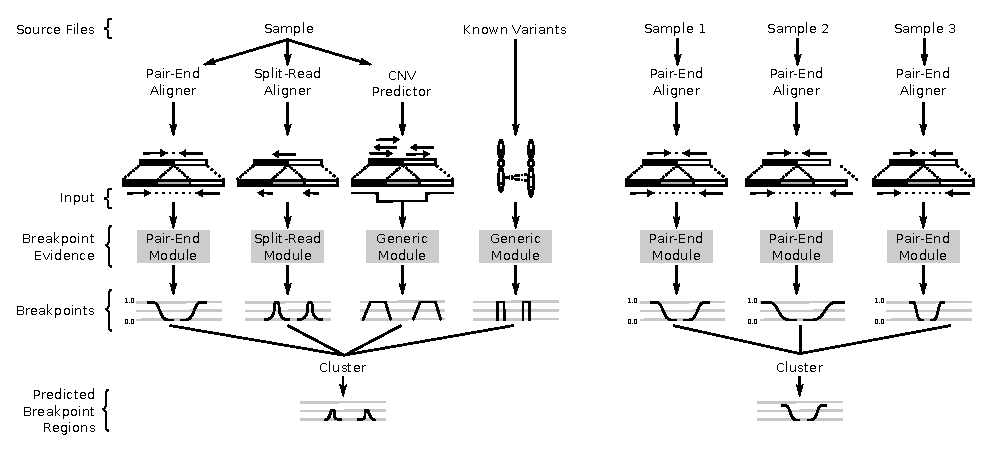
\includegraphics{img/Workflow.eps} }
    %\label{workflow:fig}
%\end{figure}
The LUMPY probabilistic SV discovery framework with two example
workflows are presented. One workflow (left) uses three different signals
(paired-end, split-read, and read-depth) from one sample, as well as prior
knowledge regarding known variant sites. The second workflow (right) integrates
a single signal type (in this case, paired-end) from three different samples to
improve discovery among sensitivity among all three samples.

\subsection*{Figure 2 - Sensitivity and false discovery rate in a whole-genome
heterogeneous sample}
%\begin{figure}
%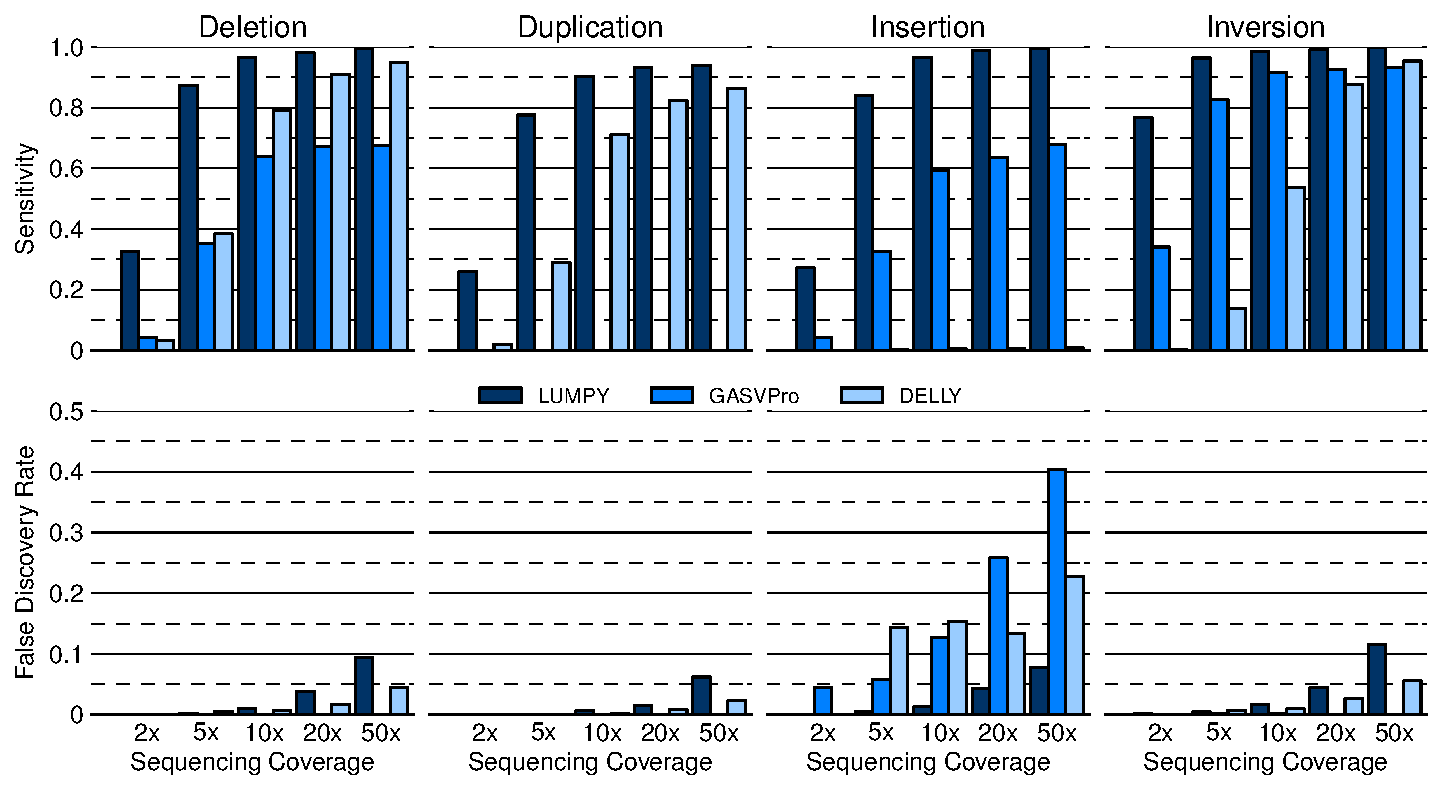
\includegraphics[width=6.5in]{graph/homozygous.eps}
%\label{sensitivity:fig}
%\end{figure}
SV discovery sensitivity and false discovery rate (FDR) for LUMPY, GASVPRO, and
DELLY for different ratios of affected to unaffected reads at different coverage
levels.

\subsection*{Figure 3 - Sensitivity and false discovery rate in a homogeneous
sample on chromosome 10}
%\begin{figure}
%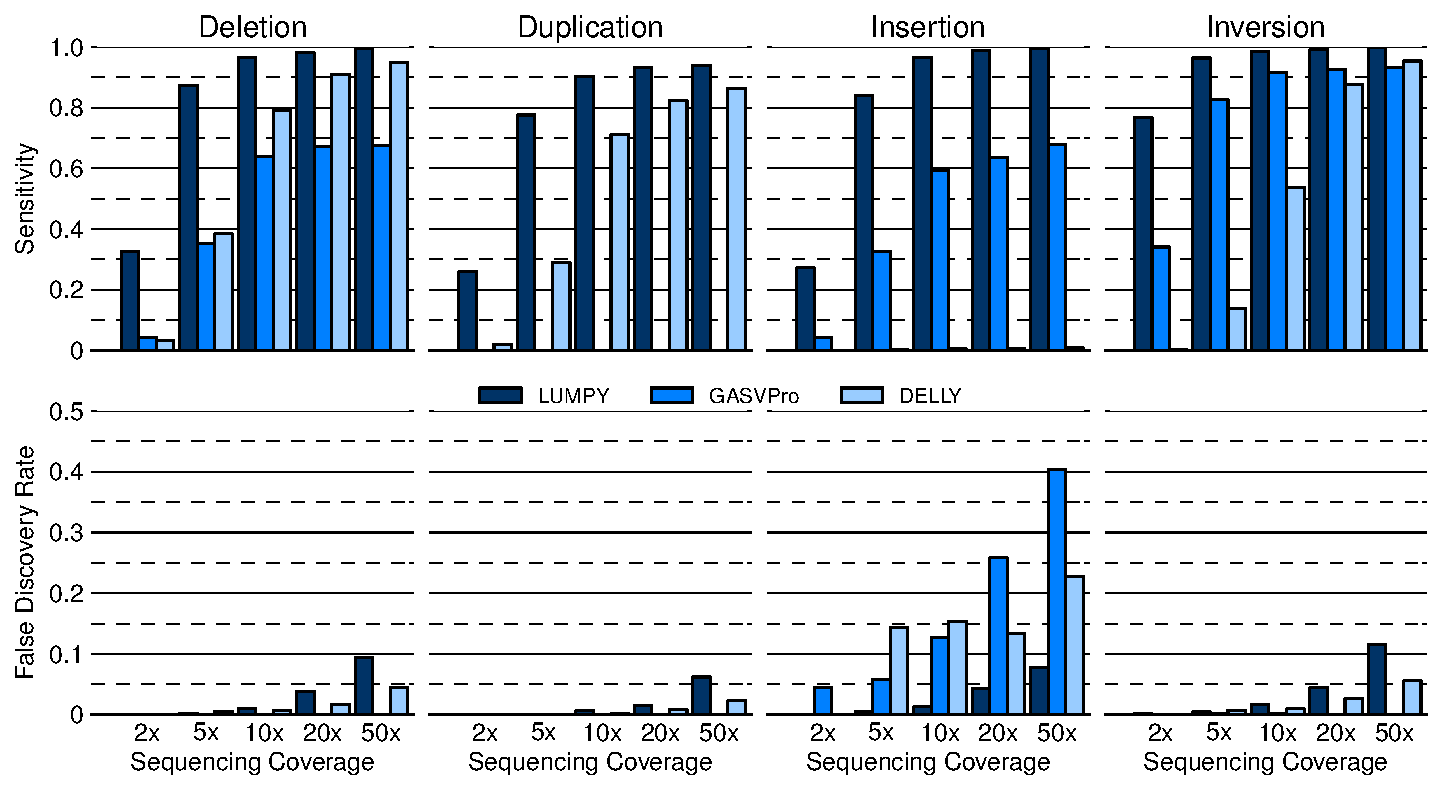
\includegraphics[width=6.5in]{graph/homozygous.eps}
%\label{sensitivity:fig}
%\end{figure}
SV discovery sensitivity and false discovery rate (FDR) for LUMPY, GASVPRO, and
DELLY for different SV types across multiple genome coverage levels.


\section*{Algorithms}

\subsection*{Paired-End Sequencing Alignments}
\label{pe:sec}
\begin{algorithm}[H]
    \DontPrintSemicolon
    \footnotesize
	\KwIn{Reference genome $R$,
		  One end of a sequence pair $z$,
		  expected fragment length $\overline{l}$
		  and standard deviation $\overline{s}$,
		  tuning parameter $v_f$,
		  fragment length cumulative distribution $D$}
    \KwOut{One end of a breakpoint interval $t$}
    \BlankLine
    \textbf{Function} $\textsc{get\_one\_bpi}$\;
		%$\textsc{get\_one\_bpi}(R,z,\overline{l},\overline{s},v_f,D)$\;
	\Begin{
		\uIf{$R(x).o = +$} {
			$t.s \gets R(z).e$\;
			$t.e \gets R(z).e + \overline{l} + v_f*\overline{s}$\;
			\For{$i = 1 \to ( t.e - t.s ) $} {
				$t.p[i] \gets D(j)$\;
			}
		}
		\uElse {
			$t.e \gets R(z).s$\;
			$t.s \gets R(z).s - (\overline{l} + v_f*\overline{s})$\;
			\For{$i = 1 \to ( l.e - l.s ) $} {
				$t.p[(t.e-t.s) - i] \gets D(j)$\;
			}
		}	
		\Return $t$\;
	}
	\caption{Breakpoint evidence function that maps one end of a sequence pair
			to one end of a breakpoint interval.}
    \label{get_one_bpi}
\end{algorithm}

\begin{algorithm}[H]
    \DontPrintSemicolon
    \footnotesize
	\KwIn{Reference genome $R$,
		  Sequence pair $\langle x,y \rangle$,
		  expected fragment length $\overline{l}$
		  and standard deviation $\overline{s}$,
		  tuning parameter $v_f$,
		  fragment length cumulative distribution $D$}
   \KwOut{Breakpoint intervals $l$ and $r$}
    \BlankLine
    \textbf{Function} $\textsc{get\_bpi}$\;
		%(R,\langle x,y \rangle,\overline{l},\overline{s},v_f,D)$\;
	\Begin{
		$l \gets \textsc{get\_one\_bpi}(R,x,\overline{l},\overline{s},v_f,D)$\;
		$r \gets \textsc{get\_one\_bpi}(R,y,\overline{l},\overline{s},v_f,D)$\;
		\Return $l,r$
	}
	\caption{Breakpoint evidence function that maps a sequence pair alignment to
			a breakpoint interval.}
    \label{get_bpi}
\end{algorithm}


\subsection*{Split-Read Alignments}
\label{sr:sec}
\begin{algorithm}[H]
    \DontPrintSemicolon
    \footnotesize
	\KwIn{Reference genome $R$,
		  Split-read pair $\langle x_i,x_{i+1} \rangle$,
		  tuning parameter $v_s$,
		  breakpoint variety $v$ }
   \KwOut{Breakpoint intervals $l$ and $r$}
    \BlankLine
    \textbf{Function} $\textsc{get\_bpi}$\;
	\Begin{
		$l_c \gets NULL$	
		$r_c \gets NULL$	

		\uIf{$v = \textsc{Inversion}$} {

			\uIf{$R(x_i).s<R(x_{i+1}).s$} {
				\lIf{$R(x_i).o=+$}
					{$l_c\gets R(x_i).e,r_c\gets R(x_{i+1}).e$}\;
				\lElse {$l_c\gets R(x_i).s,r_c\gets R(x_{i+1}).s$}\;
			} \Else {
				\lIf{$R(x_i).o=+$}
					{$l_c\gets R(x_i).s,r_c\gets R(x_{i+1}).s$}\;
				\lElse
					{$l_c\gets R(x_i).e,r_c\gets R(x_{i+1}).e$}\;
			}

		}
		\lElseIf{$v = \textsc{Deletion}$}
			{$l_c\gets R(x_i).e,r_c\gets R(x_{i+1}).s$}\;
		\lElseIf{$v = \textsc{Duplication}$}
			{$l_c\gets R(x_i).s,r_c\gets R(x_{i+1}).e$}\;

		$l.s\gets l_c - v_s, l.e\gets l_c + v_s$\;
		$r.s\gets r_c - v_s, r.e\gets r_c + v_s$\;

		$\lambda = \log(1e-10)/-v_s$\;
		\For{$i = 1 \to v_s $} {
			$l.p[i] \gets r.p[i] \gets \exp^{-\lambda(v_s - i)}$
		}
		\For{$i = v_s \to 2*v_s $} {
			$l.p[i] \gets r.p[i] \gets \exp^{-\lambda(i - v_s)}$
		}
	
		\Return $l,r$
	}
	\caption{Breakpoint evidence function that maps a sequence pair alignment to
			a breakpoint interval.}
    \label{get_bpi_sr}
\end{algorithm}
\end{bmcformat}
\end{document}
